\section{Surface Heat Balance With Moveable Insulation}\label{surface-heat-balance-with-moveable-insulation}

\subsection{Basic Heat Balance Cases}\label{basic-heat-balance-cases}

A heat balance must exist at the outside surface-air interface. The incoming conductive, convective, and radiative fluxes must sum up to zero:

\begin{equation}
Conductive + Convective + Radiative = 0
\end{equation}

In contrast to the internal surface heat balance that treats all surfaces simultaneously, the external thermal balance for each surface is performed independent of all other surfaces. This implies that there is no direct interaction between the individual surfaces.

TARP includes four possible representations for the basic outside surface heat balance. The first two depend on which of the optimal surface conductance algorithms the user selects. The simple outside surface conductance that includes both the convective and thermal interchange between the surface and the environment in a single coefficient, is represented by the thermal network in Figure~\ref{fig:thermal-network-for-simple-outside-surface}. Equation can also be expressed as:

\begin{equation}
\left[ {{\rm{KO}}{{\rm{P}}_{\rm{t}}} + {{\rm{Y}}_{\rm{0}}}\cdot {\rm{T}}{{\rm{I}}_t} - {{\rm{X}}_{\rm{0}}}\cdot {\rm{T}}{{\rm{O}}_{\rm{t}}}} \right]{\rm{ + }}\left[ {{\rm{HO}}\cdot \left( {{{\rm{T}}_{\rm{a}}} - {\rm{T}}{{\rm{O}}_t}} \right)} \right]{\rm{  + QSO  =  0}}
\end{equation}

This can be solved for the outside surface temperature.

\begin{equation}
{\rm{T}}{{\rm{O}}_{\rm{t}}}{\rm{ = }}\left[ {\frac{{{\rm{KO}}{{\rm{P}}_{\rm{t}}} + {\rm{QSO}} + {{\rm{Y}}_0}\cdot {\rm{T}}{{\rm{I}}_{\rm{t}}}{\rm{ + HO}}\cdot {{\rm{T}}_{\rm{a}}}}}{{{{\rm{X}}_{\rm{0}}}{\rm{ + HO}}}}} \right]{\rm{  }}
\end{equation}

The detailed outside surface conductance model considers convection and radiant interchange with the sky and with the ground as separate factors. Its use in the outside thermal balance is shown in Figure~\ref{fig:thermal-network-for-detailed-outside-surface}.In this case, equation can be expanded to give

\begin{equation}
\left[ {{\rm{KO}}{{\rm{P}}_{\rm{t}}}{\rm{ + }}{{\rm{Y}}_{\rm{0}}}\cdot {\rm{T}}{{\rm{I}}_{\rm{t}}}{\rm{ - }}{{\rm{X}}_{\rm{0}}}\cdot {\rm{T}}{{\rm{O}}_{\rm{t}}}} \right]{\rm{ + }}\left[ {{\rm{HA}}\cdot \left( {{{\rm{T}}_{\rm{a}}}{\rm{ - T}}{{\rm{O}}_{\rm{t}}}} \right){\rm{ + HS}}\cdot \left( {{{\rm{T}}_{\rm{s}}}{\rm{ - T}}{{\rm{O}}_{\rm{t}}}} \right){\rm{ + HG}}\cdot \left( {{{\rm{T}}_{\rm{g}}}{\rm{ - T}}{{\rm{O}}_{\rm{t}}}} \right)} \right]{\rm{  + QSO  =  0  }}
\end{equation}

This can be solved for the outside surface temperature:

\begin{equation}
{\rm{T}}{{\rm{O}}_{\rm{t}}}{\rm{ = }}\left[ {\frac{{{\rm{KO}}{{\rm{P}}_{\rm{t}}} + {\rm{QSO}} + {{\rm{Y}}_0}\cdot {\rm{T}}{{\rm{I}}_{\rm{t}}}{\rm{ + HA}}\cdot {{\rm{T}}_{\rm{a}}}{\rm{ + HS}}\cdot {{\rm{T}}_{\rm{s}}}{\rm{ + HG}}\cdot {{\rm{T}}_{\rm{g}}}}}{{{{\rm{X}}_{\rm{0}}}{\rm{ + HA + HS + HG}}}}} \right]{\rm{  }}
\end{equation}

The third and fourth representations occur when the outside surface has been covered with movable insulation. The insulation has a conductance of UM. The thermal network in Figure~\ref{fig:thermal-network-for-outside-moveable} represents this case.The insulation must be mass-less because it is not generally possible to perform a correct thermal balance at the juncture of two surfaces each modeled by CTF.

The equation for the thermal balance between the surface and the insulation is

\begin{equation}
\left[ {{\rm{KO}}{{\rm{P}}_{\rm{t}}} + {{\rm{Y}}_{\rm{0}}}\cdot {\rm{T}}{{\rm{I}}_t} - {{\rm{X}}_{\rm{0}}}\cdot {\rm{T}}{{\rm{O}}_{\rm{t}}} + {\rm{UM}}\cdot \left( {{\rm{TM - T}}{{\rm{O}}_{\rm{t}}}} \right)} \right]{\rm{ + QSO  =  0}}
\end{equation}

Which can be rewritten to solve for TO :

\begin{equation}
{\rm{T}}{{\rm{O}}_{\rm{t}}}{\rm{ = }}\left[ {\frac{{{\rm{KO}}{{\rm{P}}_{\rm{t}}} + {\rm{QSO}} + {{\rm{Y}}_0}\cdot {\rm{T}}{{\rm{I}}_{\rm{t}}}{\rm{ + UM}}\cdot {\rm{TM}}}}{{{{\rm{X}}_{\rm{0}}}{\rm{ + UM}}}}} \right]{\rm{  }}
\end{equation}

Depending on whether or not the detailed or simple algorithm for surface conductance is being used, there are two expressions for TM, the outside temperature of the insulation. For the simple conductance:

\begin{equation}
{\rm{TM}} = \left[ {\frac{{{\rm{QSM + UM}}\cdot {\rm{T}}{{\rm{O}}_{\rm{t}}}{\rm{ + HO}}\cdot {{\rm{T}}_{\rm{a}}}}}{{{\rm{UM + HO}}}}} \right]
\end{equation}

For the detailed conductance:

\begin{equation}
{\rm{T}}{{\rm{O}}_{\rm{t}}}{\rm{ = }}\left[ {\frac{{{\rm{QSM}} + {\rm{UM}}\cdot {\rm{T}}{{\rm{O}}_{\rm{t}}}{\rm{ + HA}}\cdot {{\rm{T}}_{\rm{a}}}{\rm{ + HS}}\cdot {{\rm{T}}_{\rm{s}}}{\rm{ + HG}}\cdot {{\rm{T}}_{\rm{g}}}}}{{{\rm{UM + HA + HS + HG}}}}} \right]{\rm{  }}
\end{equation}

In this case the values of HA, HS and HG must be found by using an estimated value of TM in place of TO.

\begin{figure}[hbtp] % fig 29
\centering
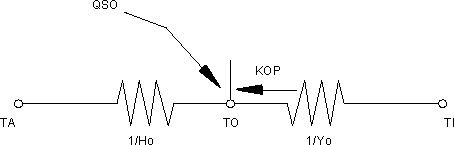
\includegraphics[width=0.9\textwidth, height=0.9\textheight, keepaspectratio=true]{media/image420.png}
\caption{Thermal Network for Simple Outside Surface Coefficient \protect \label{fig:thermal-network-for-simple-outside-surface}}
\end{figure}

\begin{figure}[hbtp] % fig 30
\centering
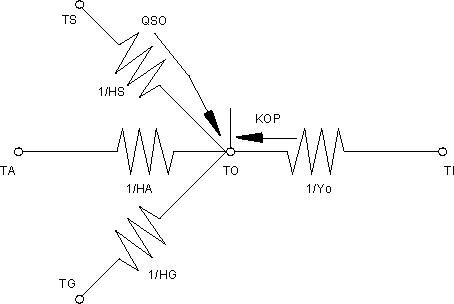
\includegraphics[width=0.9\textwidth, height=0.9\textheight, keepaspectratio=true]{media/image421.png}
\caption{Thermal Network for Detailed Outside Surface Coefficient \protect \label{fig:thermal-network-for-detailed-outside-surface}}
\end{figure}

\begin{figure}[hbtp] % fig 31
\centering
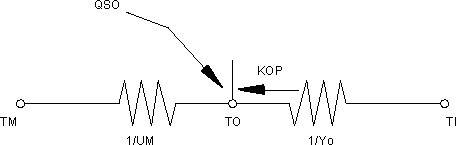
\includegraphics[width=0.9\textwidth, height=0.9\textheight, keepaspectratio=true]{media/image422.png}
\caption{Thermal Network for Outside Moveable Insulation \protect \label{fig:thermal-network-for-outside-moveable}}
\end{figure}

\subsection{Heat Balance Cases}\label{heat-balance-cases}

TO\(_{t}\) and TI\(_{t}\) are related through the Y\(_{0}\)CTF. However TI\(_{t}\) is also unknown. While it is possible to combine the outside and the inside surface heat balances to compute TO\(_{t}\) and TI\(_{t}\) simultaneously, TARP uses a simpler procedure where TO\(_{t}\) is based on a previous value of TI. When Y\(_{0}\) is small, as occurs in well insulated or very massive surfaces, TI\(_{t}\) can be replaced by TI\(_{t-1}\) (which is known for the previous hour's heat balance) without significantly effecting the value of TO\(_{t}\) When Y\(_{0}\) is large, TO and TI can so strongly be coupled that separate outside and inside heat balances do not work because the environment and zone temperatures have negligible influence on the heat balances. The TARP uses the inside surface heat balance to couple TO\(_{t}\) with TZ and TR. These two temperatures are less strongly influenced by TO and allow a reasonable heat balance. On the first heat balance iteration, TZ and TR are the values at time t-1. The user may optionally require that TO\(_{t}\) be recomputed with every iteration of TI\(_{t}\). ~In this case TZ and TR have values from the previous iteration and a true simultaneous solution is achieved. In most conventional constructions, recomputing TO\(_{t}\) does not significantly change the computed zone loads and temperatures. The inside surface heat balance is given by

\begin{equation}
{\rm{T}}{{\rm{I}}_{\rm{t}}} = \left[ {\frac{{KI{P_t} + QSI + HC\cdot TZ + HR\cdot TR + {Y_0}\cdot TO}}{{{Z_0} + HC + HR}}} \right]
\end{equation}

The surface heat balances can be combined in eight ways according to conditions for calculations of the outside surface temperature

\begin{equation}
{F_1} = \left[ {\frac{{{Y_0}}}{{{Z_0} + HI + HR}}} \right]
\end{equation}

\begin{equation}
{F_2} = \left[ {\frac{{UM}}{{UM + HO}}} \right]
\end{equation}

\begin{equation}
{F_3} = \left[ {\frac{{UM}}{{UM + HA + HS + HG}}} \right]
\end{equation}

\subsubsection{\texorpdfstring{Case1: Y\(_{0}\)~ small, simple conductance, no movable insulation:}{Case1: Y\_\{0\}~ small, simple conductance, no movable insulation:}}\label{case1-yux5f0-small-simple-conductance-no-movable-insulation}

From Equation

\begin{equation}
{\rm{T}}{{\rm{O}}_{\rm{t}}}{\rm{ = }}\left[ {\frac{{{\rm{KO}}{{\rm{P}}_{\rm{t}}} + {\rm{QSO}} + {{\rm{Y}}_0}\cdot {\rm{T}}{{\rm{I}}_{{\rm{t - 1}}}}{\rm{ + HO}}\cdot {{\rm{T}}_{\rm{a}}}}}{{{{\rm{X}}_{\rm{0}}}{\rm{ + HO}}}}} \right]{\rm{  }}
\end{equation}

\subsubsection{\texorpdfstring{Case2: Y\(_{0}\) not small, simple conductance, no movable insulation:}{Case2: Y\_\{0\} not small, simple conductance, no movable insulation:}}\label{case2-yux5f0-not-small-simple-conductance-no-movable-insulation}

From Equations and

\begin{equation}
{\rm{T}}{{\rm{O}}_{\rm{t}}}{\rm{ = }}\left[ {\frac{{{\rm{KO}}{{\rm{P}}_{\rm{t}}} + {\rm{QSO}} + {\rm{HO}}\cdot {{\rm{T}}_{\rm{a}}} + {{\rm{F}}_1}\cdot \left( {{\rm{KI}}{{\rm{P}}_{\rm{t}}}{\rm{ + QSI + HI}}\cdot {\rm{TZ + HR}}\cdot {\rm{TR}}} \right)}}{{{{\rm{X}}_{\rm{0}}}{\rm{ + HO - }}{{\rm{F}}_{\rm{1}}}\cdot {{\rm{Y}}_0}}}} \right]{\rm{  }}
\end{equation}

\subsubsection{\texorpdfstring{Case3: Y\(_{0}\)~ small, detailed conductance, no movable insulation:}{Case3: Y\_\{0\}~ small, detailed conductance, no movable insulation:}}\label{case3-yux5f0-small-detailed-conductance-no-movable-insulation}

From Equation

\begin{equation}
{\rm{T}}{{\rm{O}}_{\rm{t}}}{\rm{ = }}\left[ {\frac{{{\rm{KO}}{{\rm{P}}_{\rm{t}}} + {\rm{QSO}} + {{\rm{Y}}_0}\cdot {\rm{T}}{{\rm{I}}_{{\rm{t - 1}}}}{\rm{ + HA}}\cdot {{\rm{T}}_{\rm{a}}} + {\rm{HS}}\cdot {{\rm{T}}_{\rm{s}}} + {\rm{HG}}\cdot {{\rm{T}}_{\rm{g}}}}}{{{{\rm{X}}_{\rm{0}}}{\rm{ + HA + HS + HG}}}}} \right]{\rm{  }}
\end{equation}

\subsubsection{\texorpdfstring{Case4: Y\(_{0}\) not small, detailed conductance, no movable insulation:}{Case4: Y\_\{0\} not small, detailed conductance, no movable insulation:}}\label{case4-yux5f0-not-small-detailed-conductance-no-movable-insulation}

From Equations and

\begin{equation}
{\rm{T}}{{\rm{O}}_{\rm{t}}}{\rm{ = }}\left[ {\frac{{{\rm{KO}}{{\rm{P}}_{\rm{t}}} + {\rm{QSO}} + {\rm{HA}}\cdot {{\rm{T}}_{\rm{a}}} + {\rm{HS}}\cdot {{\rm{T}}_{\rm{s}}} + {\rm{HG}}\cdot {{\rm{T}}_{\rm{g}}} + {{\rm{F}}_{\rm{1}}}\cdot \left( {{\rm{KI}}{{\rm{P}}_{\rm{t}}}{\rm{ + QSI + HI}}\cdot {\rm{TZ + HR}}\cdot {\rm{TR}}} \right)}}{{{{\rm{X}}_{\rm{0}}}{\rm{ + HA + HS + HG - }}{{\rm{F}}_1}\cdot {{\rm{Y}}_0}}}} \right]{\rm{  }}
\end{equation}

\subsubsection{\texorpdfstring{Case5: Y\(_{0}\)~ small, simple conductance, with movable insulation:}{Case5: Y\_\{0\}~ small, simple conductance, with movable insulation:}}\label{case5-yux5f0-small-simple-conductance-with-movable-insulation}

From Equations and \(TO_t = \left[ \frac{ KOP_t + QSO + HA \cdot T_a + HS \cdot T_s + HG \cdot T_g + F_1 \cdot \left( KIP_t QS1 + HI \cdot TZ + HR \cdot TR \right) } { X_0 + HA + HS + HG - F_1 \cdot Y_0 } \right]\)

\subsubsection{\texorpdfstring{Case6: Y\(_{0}\) not small, simple conductance, with movable insulation:}{Case6: Y\_\{0\} not small, simple conductance, with movable insulation:}}\label{case6-yux5f0-not-small-simple-conductance-with-movable-insulation}

From Equations , and

\begin{equation}
{\rm{T}}{{\rm{O}}_{\rm{t}}}{\rm{ = }}\left[ {\frac{{{\rm{KO}}{{\rm{P}}_{\rm{t}}} + {\rm{QSO}} + {{\rm{F}}_2}\cdot \left( {{\rm{QSM + HO}}\cdot {{\rm{T}}_{\rm{a}}}} \right) + {{\rm{F}}_1}\cdot \left( {{\rm{KI}}{{\rm{P}}_{\rm{t}}}{\rm{ + QSI + HI}}\cdot {\rm{TZ + HR}}\cdot {\rm{TR}}} \right)}}{{{{\rm{X}}_{\rm{0}}} + {\rm{UM - }}{{\rm{F}}_{\rm{2}}}\cdot {\rm{UM - }}{{\rm{F}}_{\rm{1}}}\cdot {{\rm{Y}}_{\rm{0}}}}}} \right]{\rm{  }}
\end{equation}

\subsubsection{\texorpdfstring{Case7: Y\(_{0}\)~ small, detailed conductance, with movable insulation:}{Case7: Y\_\{0\}~ small, detailed conductance, with movable insulation:}}\label{case7-yux5f0-small-detailed-conductance-with-movable-insulation}

From Equations and

\begin{equation}
{\rm{T}}{{\rm{O}}_{\rm{t}}}{\rm{ = }}\left[ {\frac{{{\rm{KO}}{{\rm{P}}_{\rm{t}}} + {\rm{QSO}} + {{\rm{Y}}_0}\cdot {\rm{T}}{{\rm{I}}_{{\rm{t - 1}}}}{\rm{ + }}{{\rm{F}}_{\rm{3}}}\left( {{\rm{QSM + HA}}\cdot {{\rm{T}}_{\rm{a}}}{\rm{ + HS}}\cdot {{\rm{T}}_{\rm{s}}}{\rm{ + HG}}\cdot {{\rm{T}}_{\rm{g}}}} \right)}}{{{{\rm{X}}_{\rm{0}}}{\rm{ + UM - }}{{\rm{F}}_{\rm{3}}}\cdot {\rm{UM}}}}} \right]{\rm{  }}
\end{equation}

\subsubsection{\texorpdfstring{Case8: Y\(_{0}\) not small, detailed conductance, with movable insulation:}{Case8: Y\_\{0\} not small, detailed conductance, with movable insulation:}}\label{case8-yux5f0-not-small-detailed-conductance-with-movable-insulation}

From Equations , and

\begin{equation}
\medmuskip=0mu
\thinmuskip=0mu
\thickmuskip=0mu
\nulldelimiterspace=0pt
\scriptspace=0pt
{\rm{T}}{{\rm{O}}_{\rm{t}}}{\rm{ = }}\left[ {\frac{{{\rm{KO}}{{\rm{P}}_{\rm{t}}} + {\rm{QSO}} + {{\rm{F}}_1}\cdot \left( {{\rm{KI}}{{\rm{P}}_{\rm{t}}}{\rm{ + QSI + HI}}\cdot {\rm{TZ + HR}}\cdot {\rm{TR}}} \right){\rm{ + }}{{\rm{F}}_{\rm{3}}}\left( {{\rm{QSM + HA}}\cdot {{\rm{T}}_{\rm{a}}}{\rm{ + HS}}\cdot {{\rm{T}}_{\rm{s}}}{\rm{ + HG}}\cdot {{\rm{T}}_{\rm{g}}}} \right)}}{{{{\rm{X}}_{\rm{0}}}{\rm{ + UM - }}{{\rm{F}}_{\rm{3}}}\cdot {\rm{UM - }}{{\rm{F}}_{\rm{1}}}\cdot {{\rm{Y}}_{\rm{0}}}}}} \right]{\rm{  }}
\end{equation}

\subsection{Fortran Algorithm Examples}\label{fortran-algorithm-examples}

\subsubsection{\texorpdfstring{Case5: Y\(_{0}\)~ small, simple conductance, with movable insulation:}{Case5: Y\_\{0\}~ small, simple conductance, with movable insulation:}}\label{case5-yux5f0-small-simple-conductance-with-movable-insulation-1}

From Equation

\begin{lstlisting}
! Outside heat balance case: Movable insulation, slow conduction, simple convection
 F2 = DBLE(HmovInsul) / ( DBLE(HmovInsul) + DBLE(HExtSurf(SurfNum)) )
 TH(SurfNum,1,1) = (-CTFConstOutPart(SurfNum)                       &
                    +DBLE(QRadSWOutAbs(SurfNum) )                   &
           +Construct(ConstrNum)\%CTFCross(0)*TempSurfIn(SurfNum)   &
           +F2* ( DBLE(QRadSWOutMvIns(SurfNum))                     &
           + DBLE(HExtSurf(SurfNum))* DBLE(TempExt) ) )             &
           /( Construct(ConstrNum)\%CTFOutside(0) + DBLE(HmovInsul) &
          - F2* DBLE(HMovInsul))
\end{lstlisting}

\subsubsection{\texorpdfstring{Case6: Y\(_{0}\) not small, simple conductance, with movable insulation:}{Case6: Y\_\{0\} not small, simple conductance, with movable insulation:}}\label{case6-yux5f0-not-small-simple-conductance-with-movable-insulation-1}

From Equation

\begin{lstlisting}
! Outside heat balance case: Movable insulation, quick conduction, simple convection
F2 = DBLE(HmovInsul) / ( DBLE(HmovInsul) + DBLE(HExtSurf(SurfNum)) )
TH(SurfNum,1,1) = (-CTFConstOutPart(SurfNum)              &
DBLE(QRadSWOutAbs(SurfNum))                               &
+F2*( DBLE(QRadSWOutMvIns(SurfNum))                       &
+DBLE(HExtSurf(SurfNum))* DBLE(TempExt) )                 &
+F1*( CTFConstInPart(SurfNum)                             &
+ DBLE(QRadSWInAbs(SurfNum))                              &
+ DBLE(QRadThermInAbs(SurfNum))                           &
+ DBLE(HConvIn(SurfNum))*MAT(ZoneNum)                     &
+ DBLE(NetLWRadToSurf(SurfNum)) ) )                       &
/( Construct(ConstrNum)\%CTFOutside(0) + DBLE(HmovInsul)  &
-F2* DBLE(HMovInsul )- F1*Construct(ConstrNum)\%CTFCross(0) )
\end{lstlisting}

\subsubsection{\texorpdfstring{Case7: Y\(_{0}\)~ small, detailed conductance, with movable insulation:}{Case7: Y\_\{0\}~ small, detailed conductance, with movable insulation:}}\label{case7-yux5f0-small-detailed-conductance-with-movable-insulation-1}

From Equation

\begin{lstlisting}
! Outside heat balance case: Movable insulation, slow conduction, detailed convection
F2 = DBLE(HMovInsul)/ ( DBLE(HMovInsul) + DBLE(HExtSurf(SurfNum))  &
           +DBLE(HSky) + DBLE(HGround) )
TH(SurfNum,1,1) = (-CTFConstOutPart(SurfNum)                       &
+DBLE(QRadSWOutAbs(SurfNum))                                       &
+Construct(ConstrNum)\%CTFCross(0)*TempSurfIn(SurfNum)             &
+F2*( DBLE(QRadSWOutMvIns(SurfNum))                                &
+DBLE(HExtSurf(SurfNum))*DBLE(TempExt)                             &
+DBLE(HSky)*DBLE(SkyTemp)                                          &
+DBLE(HGround)*DBLE(OutDryBulbTemp) ) )                            &
/( Construct(ConstrNum)\%CTFOutside(0)                             &
+DBLE(HMovInsul) - F2*DBLE(HMovInsul) )
\end{lstlisting}

\subsubsection{\texorpdfstring{Case8: Y\(_{0}\) not small, detailed conductance, with movable insulation:}{Case8: Y\_\{0\} not small, detailed conductance, with movable insulation:}}\label{case8-yux5f0-not-small-detailed-conductance-with-movable-insulation-1}

From Equation

\begin{lstlisting}
! Outside heat balance case: Movable insulation, quick conduction, detailed convection
F2 = DBLE(HMovInsul)/ ( DBLE(HMovInsul) + DBLE(HExtSurf(SurfNum)) &
           +DBLE(HSky) + DBLE(HGround) )
TH(SurfNum,1,1) = (-CTFConstOutPart(SurfNum)                      &
+DBLE(QRadSWOutAbs(SurfNum))                                      &
+F1*( CTFConstInPart(SurfNum)                                     &
+DBLE(QRadSWInAbs(SurfNum))                                       &
+DBLE(QRadThermInAbs(SurfNum))                                    &
+DBLE(HConvIn(SurfNum))*MAT(ZoneNum)                              &
+DBLE(NetLWRadToSurf(SurfNum)) )                                  &
+F2*( DBLE(QRadSWOutMvIns(SurfNum))                               &
+DBLE(HExtSurf(SurfNum))*DBLE(TempExt)                            &
+DBLE(HSky)*DBLE(SkyTemp)                                         &
+DBLE(HGround)*DBLE(OutDryBulbTemp) )                             &
/( Construct(ConstrNum)\%CTFOutside(0)                            &
+DBLE(HMovInsul) - F2*DBLE(HMovInsul)                             &
-F1*Construct(ConstrNum)\%CTFCross(0) )
\end{lstlisting}

\subsection{Fortran Variable Descriptions}\label{fortran-variable-descriptions}

% table 16
{\scriptsize
\begin{longtable}[c]{p{1.8in}p{1.2in}p{0.9in}p{0.9in}p{1.2in}}

\caption{Fortran Variables and Descriptions \label{table:fortran-variables-and-descriptions}} \tabularnewline
\toprule 
FORTRAN Variable & Description & Tarp Variable & Units & Description \tabularnewline
\midrule
\endfirsthead

\caption[]{Fortran Variables and Descriptions} \tabularnewline
\toprule 
FORTRAN Variable & Description & Tarp Variable & Units & Description \tabularnewline
\midrule
\endhead

TH(SurfNum,1,1) & Temperature History(SurfNum,Hist Term,In/Out), where: Hist Term (1 = Current Time, 2-MaxCTFTerms = previous times), In/Out (1 = Outside, 2 = Inside) & TO & C & Temperature of outside of surface I at time t \tabularnewline
Construct(ConstrNum) \% CTFCross(0) & Cross or Y term of the CTF equation & Y0 & W/m  K & Cross CTF term \tabularnewline
Construct(ConstrNum) \% CTFInside(0) & Inside or Z terms of the CTF equation & Z0 & W/m  K & Inside CTF term \tabularnewline
Construct(ConstrNum) \% CTFOutside(0) & Outside or X terms of the CTF equation & X0 & W/m  K & Outside CTF term \tabularnewline
CTFConstInPart(SurfNum) & Constant inside portion of the CTF calculation & KIP & W/m & Portion of inward conductive flux based on previous temperature and flux history terms \tabularnewline
CTFConstOutPart(SurfNum) & Constant Outside portion of the CTF calculation & KOP & W/m & Portion of outward conductive flux based on previous temperature and flux history terms \tabularnewline
F1, F2, F3 & Intermediate calculation variables & F1, F2, F3 & ~ & Radiation interchange factor between surfaces \tabularnewline
GroundTemp & Ground surface temperature & T & C & Temperature of ground at the surface exposed to the outside environment \tabularnewline
HConvIn(SurfNum) & Inside convection coefficient & HI & W/m  K & Inside convection coefficient \tabularnewline
HExtSurf(SurfNum) & Outside Convection Coefficient & HO, HA & W/m  K & Overall outside surface conductance \tabularnewline
HGround & Radiant exchange (linearized) coefficient & HG & W/m  K & Radiative conductance (outside surface to ground temperature \tabularnewline
HmovInsul & Conductance or "h" value of movable insulation & UM & W/m  K & Conductance of Movable insulation \tabularnewline
HSky & Radiant exchange (linearized) coefficient & HS & W/m  K & Radiative conductance (outside surface to sky radiant temperature \tabularnewline
MAT(ZoneNum) & Zone temperature & TZ & C & Temperature of zone air \tabularnewline
NetLWRadToSurf(SurfNum) & Net interior longwave radiation to a surface from other surfaces & HR*TR & W/m & Net surface to surface radiant exchange \tabularnewline
QRadSWInAbs(SurfNum) & Short-wave radiation absorbed on inside of opaque surface & QSI & W/m & Short wave radiant flux absorbed at inside of surface \tabularnewline
QRadSWOutAbs(SurfNum) & Short wave radiation absorbed on outside opaque surface & QSO & W/m & Short wave radiant flux absorbed at outside of surface \tabularnewline
QRadSWOutMvIns(SurfNum) & Short wave radiation absorbed on outside of movable insulation & QSM & W/m & Short wave radiant flux absorbed at surface of movable insulation \tabularnewline
QRadThermInAbs(SurfNum) & Thermal Radiation absorbed on inside surfaces & ~ & W/m & Longwave radiant flux from internal gains \tabularnewline
SkyTemp & Sky temperature & T & C & Sky temp \tabularnewline
TempExt & Exterior surface temperature or exterior air temperature & TM, T & C & Temperature of external surface of movable insulation or outside ambient air temperature \tabularnewline
TempSurfIn(SurfNum) & Temperature of inside surface for each heat transfer surface & TI & C & Temperature of inside of surface I at time t-1 \tabularnewline
\bottomrule
\end{longtable}}

\subsection{References}\label{references-044}

Walton, G.N. 1983. ``The Thermal Analysis Research Program Reference Manual Program (TARP)'', National Bureau of Standards (now National Institute of Standards and Technology).
